\chapter{Betanítás}
\label{ch:training}

\section{Tanítóadatok}

A betanításhoz 29 romániai hulladéklerakó és közvetlen környezete került a tanítóadatok közé, illetve a Kiskörei víztároló is. A víztároló már vizsgálva volt \cite{magyar2023}-ban, és alkalmas úszó hulladéksziget detektálására, tekintve arra, hogy a felgyült faágak között nagy koncentrációban jelenik meg műanyag-alapú hulladék. A \ref{fig:kiskore-waste} ábrán látható, hogy miként gyűl össze a hulladék a víztárolónál. A romániai hulladéklerakókat egy helyi weboldalon lehet megtalálni, a hozzájuk tartozó koordinátákkal együtt \cite{wasteromania2019}. Az ott bemutatott 46 hulladéklerakó közül 29 volt alkalmas tanításra: sok hulladéklerakó be lett tömve, vagy föld alatt működik. Minden hulladéklerakóhoz letöltöttem egy-egy nyári+tavaszi, téli és őszi multispektrális műholdképet, melyeket kézzel annotáltam. A nyári és tavaszi képeket azért vontam egybe, mivel ezek hulladékdetektálás szempontjából hasonló adatokat eredményeztek. A tanítóadatok pixelenként vannak előállítva, így a végső adathalmaz 27 millió tanítóadatból (pixelből) áll. Minden pixelhez hozzá van rendelve a vörös, kék, zöld, közeli infravörös sáv, illetve a "PI", "NDWI", "NDVI", "RNDVI", "SR" indexek. Ezen felül minden pixel címkézve van a \ref{tab:waste-detection-labels} táblázatban leírtak szerint. Nagyon fontos, hogy minél pontosabban meg lehessen állapítani, hogy a hulladéklerakókon mely területeken található hulladék, hiszen sok hulladéklerakón törmeléket is tárolnak, ezt általában egy külön területen. Emiatt a tanítóadatokat a következő módszerrel állítottam elő: Megvizsgáltam Google Maps segítségével \cite{googlemaps2024}, hogy az adott hulladéklerakónál hol tárolnak törmeléket és hol tárolnak műanyag alapú hulladékot. A Google Maps légi felvételei elég magas felbontással rendelkeznek ahhoz, hogy általában szemmel meglehessen különböztetni a műanyag alapú hulladékot a törmeléktől. A \ref{fig:waste-vs-debris} ábrából látható, hogy míg a törmelék inkább fehér színt tartalmaz, addig a műanyag alapú hulladék picit vörösebb, tekintve arra, hogy a műanyag sokszor színezve van. Emellett, a hulladéklerakókat nagyon konzervatívan jelöltem ki: csak akkor jelöltem be egy területet, mint hulladékos terület, ha a felvételből egyértelmű volt, hogy az adott terület műanyag alapú hulladékkal szennyezett. Természetesen, helyi terepvizsgálattal, illetve magasabb felbontású felvételek készítésével pontosabb adatokat lehetne előállítani. 

\begin{figure}[H]
	\centering
	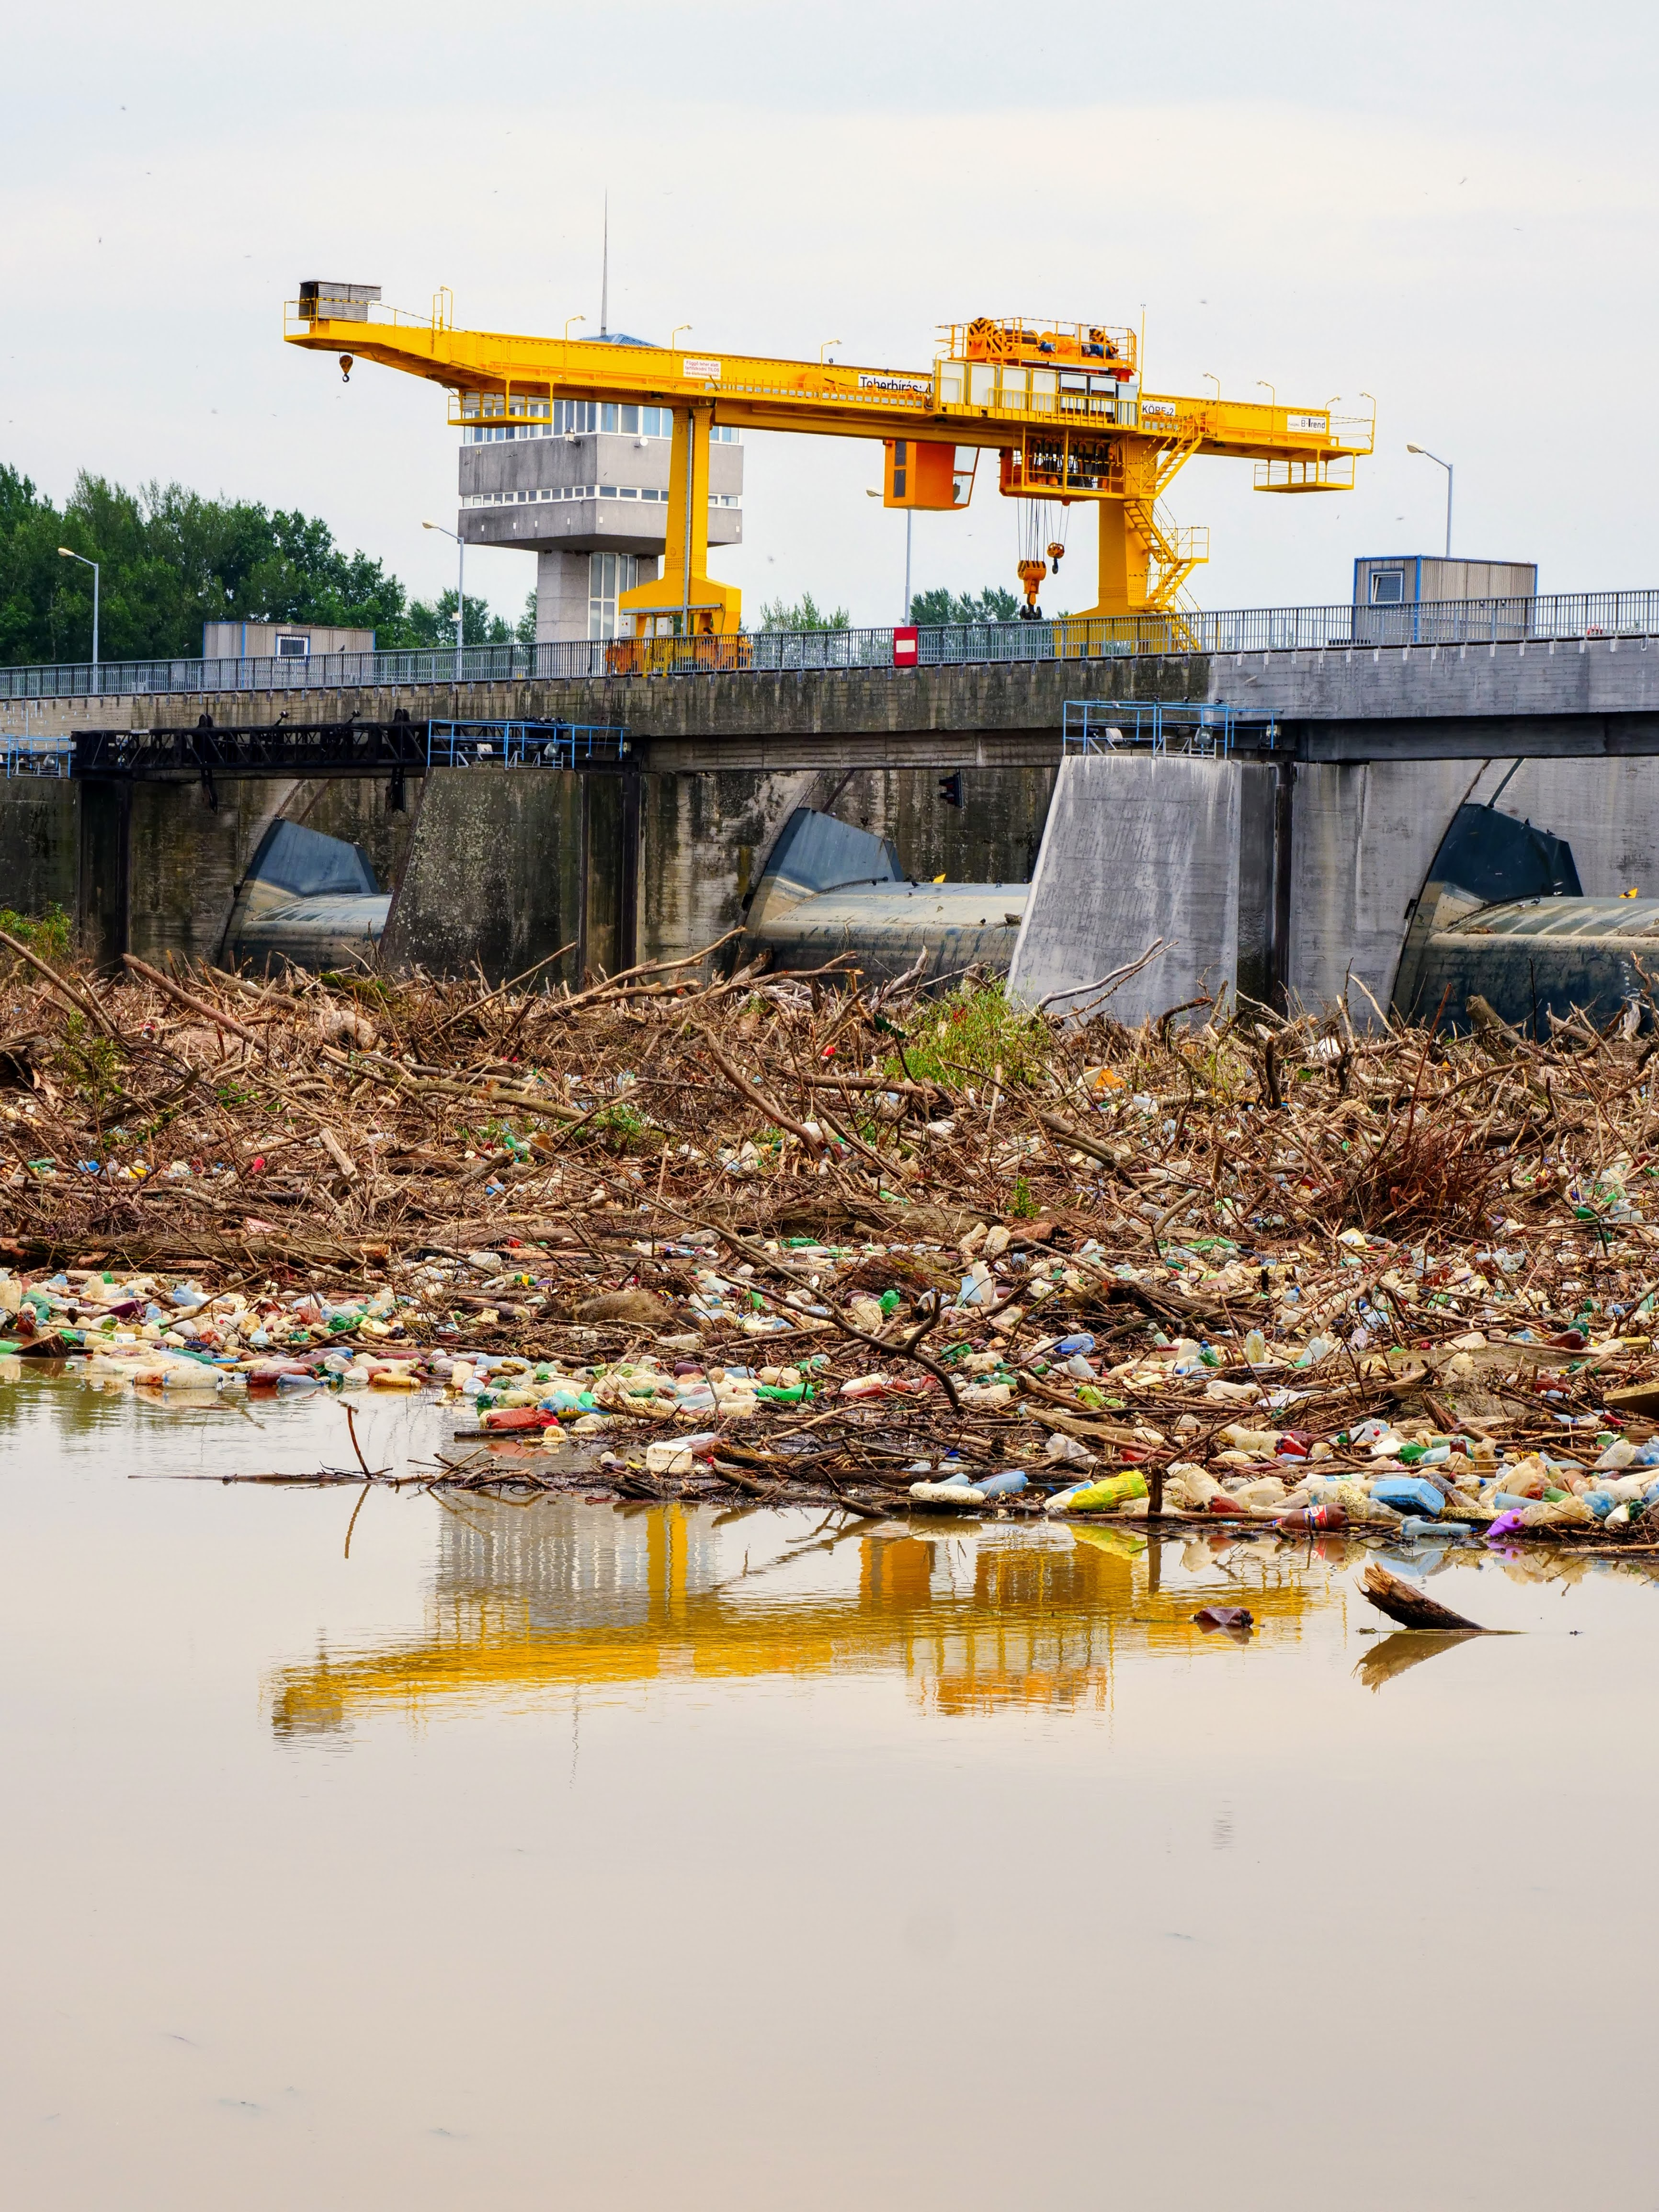
\includegraphics[width=0.6\textwidth,frame]{kiskore-garbage}
	\caption{A kiskörei víztároló hulladéktorlasza \cite{petkupa2024}}
    \label{fig:kiskore-waste}
\end{figure}

\begin{table}[H]
	\centering
	\begin{tabular}{ | p{0.1\textwidth} | p{0.2\textwidth} | p{0.6\textwidth} | }
		\hline
		\textbf{Címke azonosító} & \textbf{Címke neve} & \textbf{Címke magyarázat} \\
		\hline \hline
		\emph{100} & Hulladék & Azon területek, melyeken hulladékot találtunk. \\
		\hline
		\emph{200} & Víz & olyan területek, melyeken kizárólag vizet találtunk, általában folyók. \\
		\hline
		\emph{300} & Legelők/Erdők & Zöld övezetből álló vad területek. Ezek lehetnek fák lombjai vagy füves zónák. \\
		\hline
        \emph{400} & Mezők & Olyan földes területek, melyek meg vannak művelve, illetve ahol mezőgazdasági növények találhatóak, például gabonafélék. \\
		\hline
        \emph{500} & Ismeretlen & Olyan területek, melyek a korábbi kategóriákba nem sorolhatók bele. Ilyenek az épületek, aszfaltozott utak, háztetők, mezei utak. \\
		\hline
	\end{tabular}
	\caption{A tanítóadatok címkéi}
	\label{tab:waste-detection-labels}
\end{table}

\begin{figure}[H]
	\centering
	\subcaptionbox{Műanyag alapú hulladék}{
		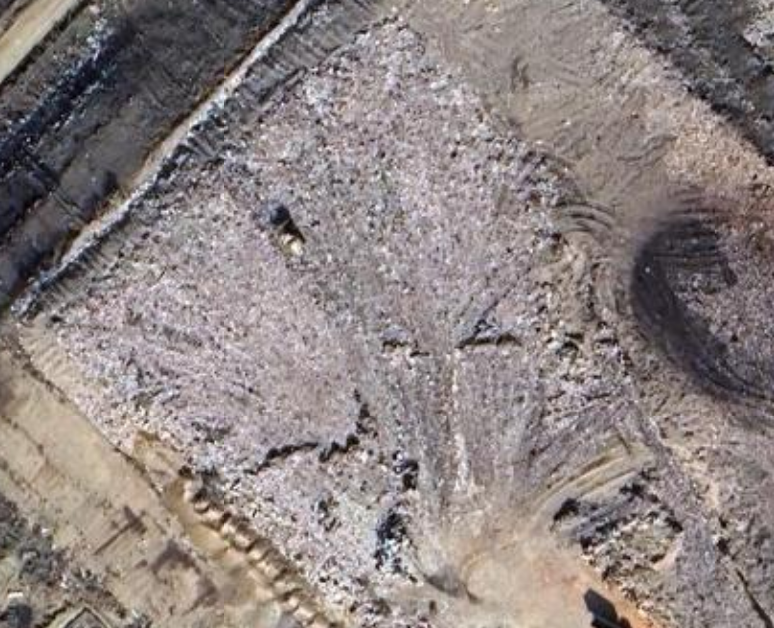
\includegraphics[width=0.45\linewidth]{waste}}
	\hspace{5pt}
	\subcaptionbox{Törmelék}{
		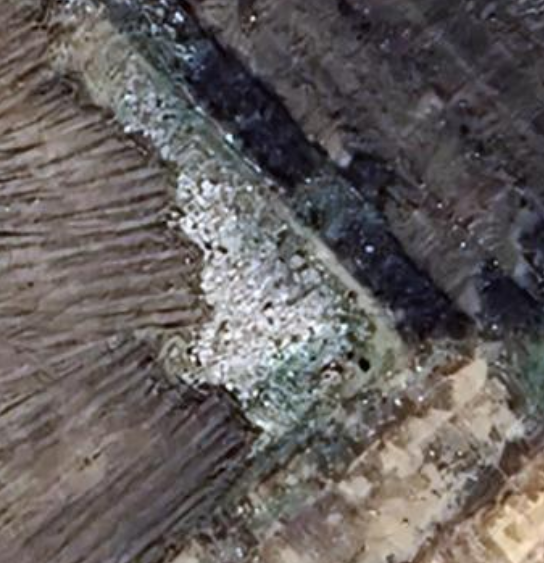
\includegraphics[width=0.45\linewidth]{debris}}
	\caption{A műanyag alapú hulladék, törmelék mellé helyezve. Forrás: Google Maps}
	\label{fig:waste-vs-debris}
\end{figure}



\section{Tanítási paraméterek}
\label{ch:teaching-params}

A nagy adathalmaz miatt a Random Forest modell is nagyon nagy lesz (körülbelül 14GB), ami egy nehezen kezelhető méret, így érdemes módosítani a modell paraméterein, hogy ez kisebb méretű legyen. A legjobb eredményeket azzal értem el, hogy a Random Forest fák méretét 20 mélységűre limitáltam. Ennek köszönhetően a modellek méretét 2GB-ra tudtam csökkenteni \todo{táblázat a fák méretéről, a modellek méretéről és a különböző mélységekről}, és a \ref{fig:fullsize-vs-reduced} ábrából látható, hogy a csökkentett modellben enyhén megnő a hulladékra vonatkozó false-negative ráta, míg a false positive arány nem nő, de cserében egy kezelhető méretű modellt kapunk.

\begin{figure}[H]
	\centering
  \subcaptionbox{A klasszifikálandó felvétel}{
		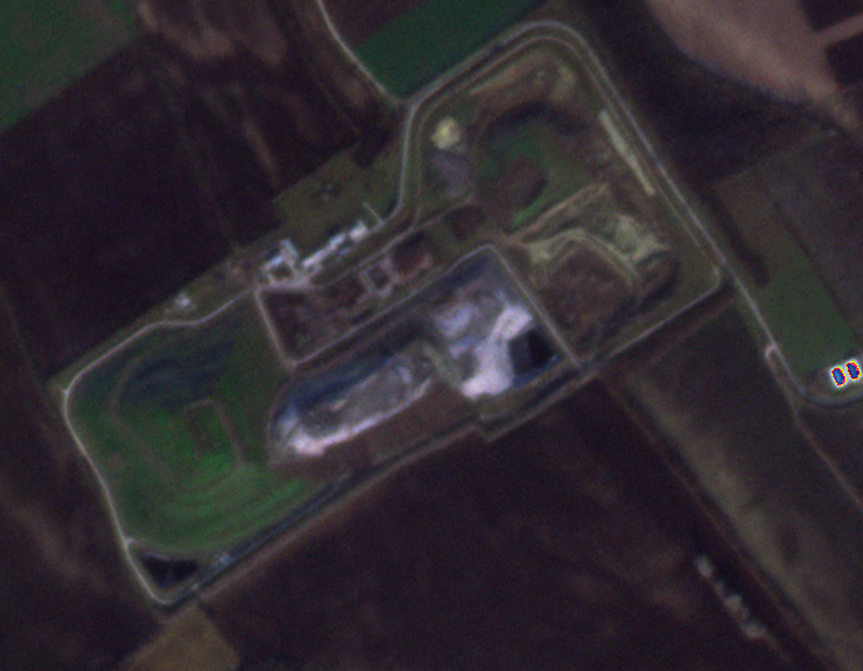
\includegraphics[width=0.45\linewidth]{original-pusztazamor}}
	\hspace{5pt}
	\subcaptionbox{Teljes méretű modell}{
		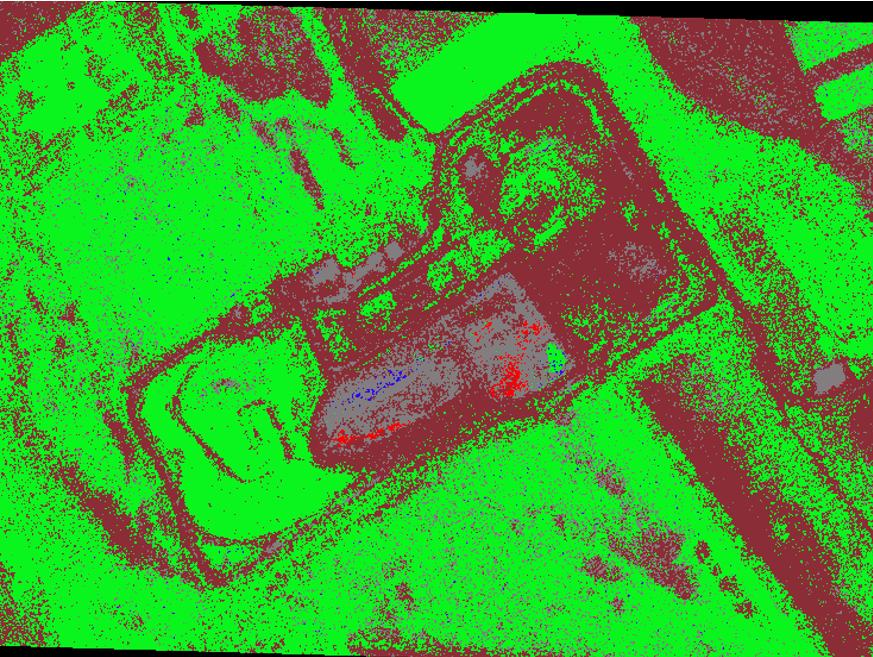
\includegraphics[width=0.45\linewidth]{fullsized}}
	\hspace{5pt}
	\subcaptionbox{Csökkentett modell}{
		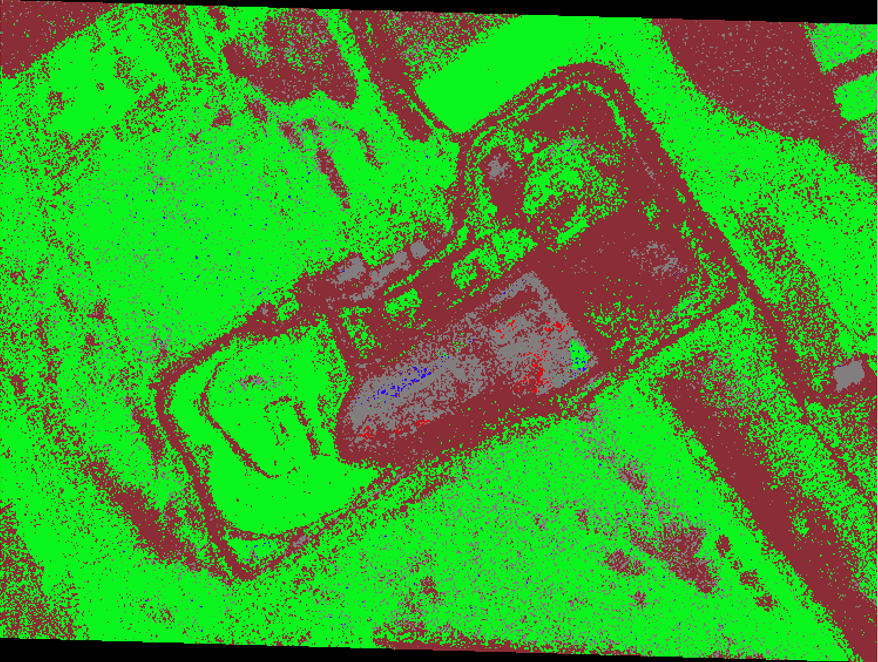
\includegraphics[width=0.45\linewidth]{reduced}}
	\caption{A csökkentett modell hasonlóan teljesít a teljes méretű modellhez}
	\label{fig:fullsize-vs-reduced}
\end{figure}

Továbbiakban felmerült az a probléma is, hogy a tanítóadatok nagyon aránytalanok voltak: A \ref{fig:unbalanced-data} ábrából látható, hogy nagyságrendekkel kevesebb adattal rendelkeztünk hulladékról, mint az összes többi adatról. Emiatt a modell nagyon sok false-negatív-ot termelt. Ennek korrigálására súlyokat alkalmaztam a tanítóadatokra. A súlyok kiszámolásához az összes címkére a \ref{eq:weights} képletet használtam.

\pgfplotstableread[row sep=\\,col sep=&]{
    label           & value     \\
    Hulladék        & 29513     \\
    Víz             & 926356    \\
    Legelők/Erdők   & 12573615  \\
    Mezők           & 8043948   \\
    Ismeretlen      & 5669416   \\
}\datacounts

\begin{figure}
    \begin{tikzpicture}
        \begin{axis}[
                ybar,
                ymode = log,
                bar width=1cm,
                width=\textwidth,
                height=0.5\textwidth,
                symbolic x coords={Hulladék,Víz,Legelők/Erdők,Mezők,Ismeretlen},
                xtick=data,
            ]
            \addplot table[x=label,y=value]{\datacounts};
        \end{axis}
    \end{tikzpicture}
    \caption{Az adatok közötti aránytalanság, logaritmikus skálázással}
    \label{fig:unbalanced-data}
\end{figure}

\begin{equation}\label{eq:weights}
    c\acute{\imath}mke \ s\acute{u}lya=\frac{adathalmaz \ m\acute{e}rete}{c\acute{\imath}mke \ darabsz\acute{a}ma}
\end{equation}

\section{Felvételek normalizálása}
Az egyik legnagyobb kihívás az Random Forestnek az, hogy hogyha elég nagy eltérések vannak a felvételek között, például időjárás miatt, akkor hajlandó félreosztályozni egyes területeket. Ennek korrigálára érdemes megvizsgálni a műholdfelvételek normalizálását. A normalizálás egy referencia kép szerint történik: kiválasztok egy referencia felvételt egy adott területről és időszakról (nyár, tél), és az összes többi felvételt arról a területről és időszakról erre a felvételre normalizálom. Így a nagymértékű eltérések csökkentve lesznek a modell számára, és várhatóan jobban fogja osztályozni a felvételeket \todo{ábra, numerikus eredmények, módszer részletezése?}. 

\section{Főkomponens analízis (PCA)}
\label{ch:pca-methodology}

A modell méretének a csökkentésére megvizsgáltam a főkomponens analízis (PCA) alkalmazását is \cite{pca2010}. A főkomponens analízis a gépi tanulásban egy szélesen elterjedt módszer.  A módszer lényege az, hogy egy többdimenziós adathalmazból kivonja a legfontosabb információkat egy alacsonyabb dimenziószámú adathalmazba. Ezeket nevezzük főkomponenseknek. A főkomponensek korrelálatlanok, vagyis a korrelációs mátrixuknak a főátlóján helyezkednek el, illetve a megfigyelési egységek varianciájának a nagy részét az első pár főkomponensben tároljuk \cite{elek2011}. Azt, hogy hány főkomponenst szeretnénk megtartani, empirikus módon meghatározhatjuk annak függvényében, hogy mekkora mértékben szeretnénk megtartani az eredeti adathalmaz varianciáját. A \ref{fig:pca-variance} ábrán látható, hogy ennek az adathalmaznak az esetében ha 90\%-át szeretném megtartani a varianciának, akkor elég az első három főkomponenst megválasztanom.

\pgfplotstableread[row sep=\\,col sep=&]{
    label           & value     \\
    PC1        & 6.673e+01     \\
    PC2             & 2.239e+01    \\
    PC3   & 6.859e+00  \\
    PC4           & 2.032e+00   \\
    PC5     & 1.501e+00    \\
    PC6 & 4.057e-01    \\
    PC7 & 8.222e-02    \\
    PC8 & 5.806e-13    \\
    PC9 & -9.228e-27    \\
}\varianceretention

\begin{figure}
    \begin{tikzpicture}
        \begin{axis}[
                ybar,
                ylabel=megtartott variancia(\%),
                bar width=1cm,
                width=\textwidth,
                height=0.5\textwidth,
                symbolic x coords={PC1,PC2,PC3,PC4,PC5,PC6,PC7,PC8,PC9},
                xtick=data,
            ]
            \addplot table[x=label,y=value]{\varianceretention};
        \end{axis}
    \end{tikzpicture}
    \caption{A főkomponensek varianciája a tanítóhalmazon. 90\% variancia megtartásának érdekében elég az első három főkomponenst kiválasztani}
    \label{fig:pca-variance}
\end{figure}

A PCA használatának a motivációja az volt, hogy a bemeneti adatok dimenziószámának a csökkentésével csökkenni fog a modell mérete, de érdekes módon a modell mérete nem csökkent a dimenziószám csökkentésével, helyette lényegesen megnőtt. Ezt az is tükrözi, hogy megnőtt átlagosan a Random Forest döntési fáinak a mérete, minél kevesebb dimenziószámú adatot kapott. A \ref{tab:increase-in-model-size} táblázatból látható, hogy különböző főkomponenseknél mekkora volt átlagban a fák mérete az adatok dimenziószámának függvényében. További vizsgálatok után kiderült, hogy hogyha kevesebb dimenziójú adatot adtam a modellnek, akkor a mérete lényegesen megnőtt. 

Ezen felül az is célja volt a PCA alkalmazásának, hogy a kiszámolt indexek információit megtartva, alacsonyabb dimenziószám segítségével a Random Forest modell hatékonyabban fogja majd feldolgozni a műholdfelvételeket. \cite{Howley2005} megmutatja, hogy egyes modelleken jobb klasszifikációt tudtak elérni több spektrális sávból álló adat esetén. Ennek az az oka, hogy ha igen sok a korreláció a különböző dimenziók között, akkor a modell rátanulhat a zajra. Mivel a modell által használt indexek között sok a korreláció, érdemes megvizsgálni a PCA-t olyan szempontból is, hogy esetleg javít-e a klasszifikációs eredményeken. 

\begin{table}[H]
	\centering
	\begin{tabular}{ | p{0.3\textwidth} | p{0.3\textwidth} | }
		\hline
		\textbf{Főkomponensek száma} & \textbf{Fák méretének mediánja} \\
		\hline \hline
		Főkomponensek nélkül (9 dimenzió) & 71.5 \\
		\hline
    5 főkomponens & 71 \\
		\hline
		4 főkomponens & 73\\
		\hline
    3 főkomponens & 85 \\
    \hline
	\end{tabular}
	\caption{A döntési fák méretének a mediánja nem csökkent, amint a főkomponensek száma csökkent, cserében 3 főkomponensnél már nőtt.}
	\label{tab:increase-in-model-size}
\end{table}

A PCA alkalmazása a Random Forestre a következő lépésekből áll:
\begin{enumerate}
	\item A tanítóadatok standard skálázása a \ref{eq:standard-scaling} képlet szerint.
	\item A főkomponens analízis alkalmazása a tanítóadatokra.
	\item A Random Forest modell betanítása a tanítóadatokon.
\end{enumerate}
A főkomponens analízis folyamatának a geometriai jelentését a \ref{fig:elek-pca} ábra illusztrálja.

\begin{equation}\label{eq:standard-scaling}
  f(x) = \frac{x - Average}{Standard \ Deviation}
\end{equation}

\begin{figure}[H]
	\centering
	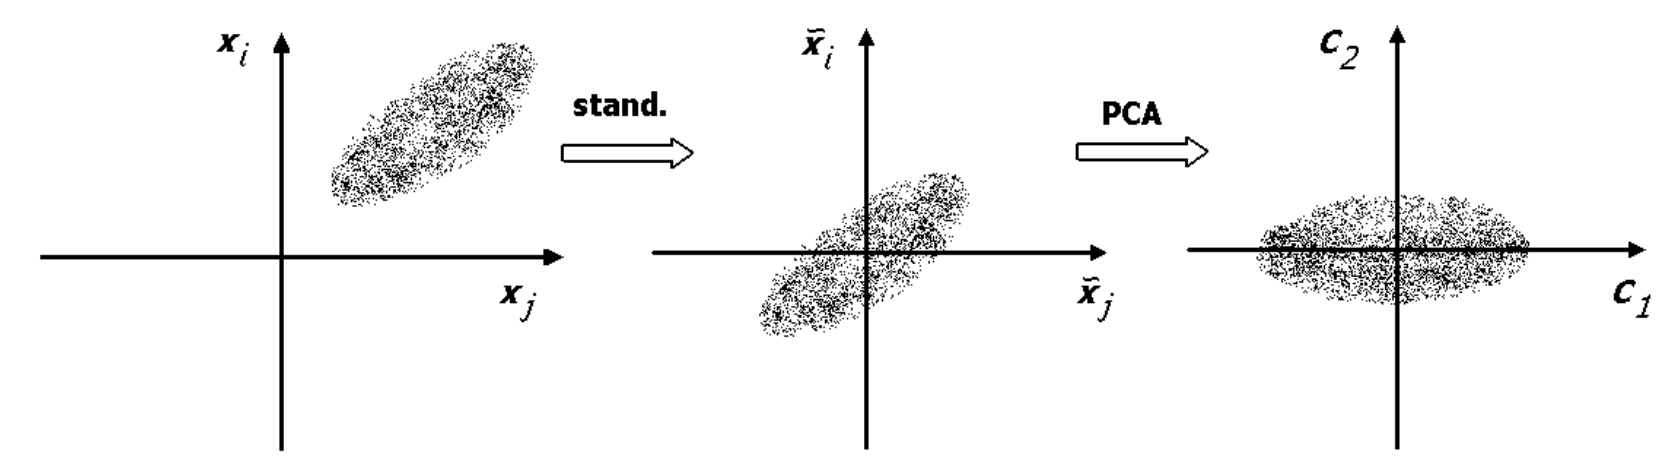
\includegraphics[width=\textwidth,frame]{elek_pca}
	\caption{A főkomponens analízis geometriai jelentése: a standardizálás 0 várható értékűvé és
  1 empirikus szórásúvá teszi a változókat, vagyis a pontfelhőt betolja az origóba,
  majd elforgatja a legnagyobb variancia irányába, ami az első főkomponens \cite{elek2011}}
    \label{fig:elek-pca}
\end{figure}

A modell tesztelésére is ugyanezeket lépéseket kell elvégezni. A főkomponens analízis használásához a scikit-learn \cite{scikit-learn} Python programcsomagot használtam. A főkomponenssel betanított modellt a \ref{ch:teaching-params} fejezetben részletezem. A \ref{ch:pca-performance} fejezetben részletezem a főkomponens analízissel tanított modell teljesítményét.

\section{Nyári és téli adatokra való lebontás}

Alapértelmezetten a nyári és téli adatok között lényeges különbség tud lenni távérzékelés szempontból Közép-Európa területén: a téli időszakokban gyérebb a vegetáció, ködösebb a levegő, illetve a nap sem süt ugyanabból a szögből. Ez befolyásolhatja a modell pontosságát is az adott időszakokban. A nyári időszakot márciustól októberig tartó időszakként definiáltam, és a téli időszak pedig novembertől februárig tart. Az időszakok aszerint vannak megválasztva, hogy mikor leveleznek ki, illetve hullatják ki a leveleiket a fák. Valóban, az októberi időszakban már inkább sárgásak lesznek a levelek, de az októberi tanítóhalmaz mérete önmagában igen kicsi érdemi tanításra. A \ref{fig:winter-vs-summer} ábrából látható, hogy főleg a közeli infravörös (NIR) sávokon nagy eltérések vannak a nyári és téli felvételek között. Ennek fényében betanítottam külön egy nyári és egy téli modellt, melyek teljesítményét a \ref{ch:summer-winter-models} \todo{fejezet elkészítése} fejezetben részletezem.

\begin{figure}
    \begin{tikzpicture}
        \begin{axis}
          [
          title={Téli felvételek értékei},
          boxplot/draw direction=y,
          ytick={0,2000,4000,6000},
          ymax={8000},
          xtick={1,2,3,4},
          xticklabels={Kék, Zöld, Piros, NIR},
          ]
          \addplot+[
          boxplot prepared={
            median=428,
            upper quartile=563,
            lower quartile=315,
            upper whisker=935,
            lower whisker=44
          },
          ] coordinates {};
          \addplot+[
          boxplot prepared={
            median=530,
            upper quartile=695,
            lower quartile=385,
            upper whisker=1160,
            lower whisker=1
          },
          ] coordinates {};
          \addplot+[
          boxplot prepared={
            median=674,
            upper quartile=923,
            lower quartile=497,
            upper whisker=1562,
            lower whisker=22
          },
          ] coordinates {};
          \addplot+[
            boxplot prepared={
              median=1629,
              upper quartile=2067,
              lower quartile=1273,
              upper whisker=3258,
              lower whisker=82
          },
          ] coordinates {};
        \end{axis}
      \end{tikzpicture}
      \begin{tikzpicture}
        \begin{axis}
          [
          title={Nyári felvételek értékei},
          boxplot/draw direction=y,
          ytick={0,2000,4000,6000},
          ymax={8000},
          yticklabel=\empty,
          xtick={1,2,3,4},
          xticklabels={Kék, Zöld, Piros, NIR},
          ]
          \addplot+[
          boxplot prepared={
            median=360,
            upper quartile=638,
            lower quartile=214,
            upper whisker=1274,
            lower whisker=1
          },
          ] coordinates {};
          \addplot+[
          boxplot prepared={
            median=578,
            upper quartile=862,
            lower quartile=415,
            upper whisker=1532,
            lower whisker=1
          },
          ] coordinates {};
          \addplot+[
          boxplot prepared={
            median=579,
            upper quartile=1058,
            lower quartile=270,
            upper whisker=2240,
            lower whisker=1
          },
          ] coordinates {};
          \addplot+[
            boxplot prepared={
              median=2850,
              upper quartile=3830,
              lower quartile=2103,
              upper whisker=6420,
              lower whisker=1
          },
          ] coordinates {};
        \end{axis}
      \end{tikzpicture}
    \caption{Nyári és téli adatok összehasonlítása}
    \label{fig:winter-vs-summer}
\end{figure}